%%%% IACR Transactions TEMPLATE %%%%
% This file shows how to use the iacrtrans class to write a paper.
% Written by Gaetan Leurent gaetan.leurent@inria.fr (2020)
% Public Domain (CC0)


%%%% 1. DOCUMENTCLASS %%%%
\documentclass[journal=tosc,preprint]{iacrtrans}
%%%% NOTES:
% - Change "journal=tosc" to "journal=tches" if needed
% - Change "submission" to "final" for final version
% - Add "spthm" for LNCS-like theorems


%%%% 2. PACKAGES %%%%
\usepackage{lipsum} % Example package -- can be removed
\usepackage{listings}
\usepackage{graphicx}
\usepackage{subcaption}

%%%% 3. AUTHOR, INSTITUTE %%%%
\author{}
\institute{
  Kriti Gupta, 12140940, \email{kritig@iitbhilai.ac.in}
  \and
  Siddhi Agarwal, 12141570, \email{siddhiag@iitbhilai.ac.in}
}
%%%% NOTES:
% - We need a city name for indexation purpose, even if it is redundant
%   (eg: University of Atlantis, Atlantis, Atlantis)
% - \inst{} can be omitted if there is a single institute,
%   or exactly one institute per author


%%%% 4. TITLE %%%%
\title{RECTANGLE CIPHER}
%%%% NOTES:
% - If the title is too long, or includes special macro, please
%   provide a "running title" as optional argument: \title[Short]{Long}
% - You can provide an optional subtitle with \subtitle.

\begin{document}

\maketitle

%%%% 5. KEYWORDS %%%%
\keywords{bit-slice implementation, lightweight block cipher, software efficiency, security analysis}


%%%% 6. ABSTRACT %%%%
\begin{abstract}
  The Rectangle Cipher is a lightweight block cipher that leverages a bit-slice-style implementation and an SP-network design, enabling efficient and fast execution. Its bit-slice architecture contributes to its lightweight nature and ensures exceptional performance across both software and hardware platforms. The cipher features sixteen parallel 4×4 S-Boxes in its substitution layer and three rotations in its permutation layer, which collectively enhance its flexibility and adaptability for various applications.\\
  The Rectangle Cipher achieves efficient hardware performance while maintaining one of the fastest software execution speeds among existing lightweight ciphers. Its robust security is a result of carefully selected S-Boxes and an asymmetric permutation layer design, providing resilience against cryptanalytic attacks. Comprehensive security analysis shows that a maximum of 18 out of the 25 rounds can be successfully attacked.
\end{abstract}


%%%% 7. PAPER CONTENT %%%%
\section{Introduction}

Small embedded devices, such as RFIDs, sensor nodes, and smart cards, are increasingly deployed across a variety of applications. These devices are subject to stringent cost constraints, including hardware limitations like area, power, and energy consumption, as well as software requirements such as low memory usage and compact code sizes. Despite these constraints, robust cryptographic protection is essential to ensure their security. Lightweight ciphers have thus emerged as cost-effective solutions, offering strong security with minimal resource consumption. Symmetric-key block ciphers, in particular, play a critical role in securing these devices, making the design of lightweight block ciphers a highly active area of research.

Numerous lightweight block ciphers employing diverse design strategies have been proposed, including PRESENT, SPECK and LED. Among these, PRESENT gained significant attention for its simplicity, strong security, and exceptional hardware performance. It employs a bit permutation in its diffusion layer, ensuring cost-effective hardware implementation. However, PRESENT and other ciphers like KATAN and Hummingbird, while efficient in hardware, often suffer from performance bottlenecks in software implementations, particularly in their diffusion layers. This dual demand for high hardware and software efficiency has driven the search for new approaches in lightweight cipher design.

The bit-slice technique, introduced to improve the software efficiency of DES, has demonstrated significant potential in achieving high software performance for symmetric ciphers. This method aligns software logical instructions with the simultaneous execution of multiple hardware logical gates, as seen in the Serpent block cipher, which uses 32 parallel 4×4 S-Boxes in its substitution layer. Ciphers like SHA-3, Trivium, and JH have also leveraged bit-slice implementations, achieving strong performance across both hardware and software while enhancing resistance to implementation attacks such as timing and cache-based attacks. However, these bit-slice-oriented designs were not explicitly tailored for lightweight applications, leaving room for improvement in crafting dedicated lightweight bit-slice ciphers.

To address these limitations, the RECTANGLE cipher was introduced. RECTANGLE is an SP-network-based lightweight block cipher that uses the bit-slice technique to achieve both high software efficiency and low-cost hardware implementation. It features sixteen parallel 4×4 S-Boxes in its substitution layer and three rotations in its permutation layer, creating an asymmetric design that enhances its security. RECTANGLE excels in hardware compactness, delivering highly competitive software speeds while maintaining robust security. Its carefully selected S-boxes and asymmetric permutation layer ensure resilience against clustering of linear and differential trails, distinguishing it from earlier lightweight designs such as PRESENT. These attributes make RECTANGLE a highly efficient and secure solution for resource-constrained embedded systems.

\section{Implementation}
 The RECTANGLE cipher is structured around a 4×16 rectangular array, representing a block length of 64 bits. It supports key lengths of either 80 or 128 bits, depending on the security requirements. The cipher operates over 25 rounds, with each round consisting of three core operations: AddRoundKey (ARK), SubColumn (SC), and ShiftRow (SR). These operations are designed to ensure strong diffusion and confusion throughout the encryption process.\\
 After completing the 25 rounds, a final AddRoundKey operation is performed to generate the ciphertext block. The cipher's simplicity and efficiency make it highly suitable for lightweight cryptographic applications.\\
 The pseudocode for the RECTANGLE Cipher is given below-
\begin{lstlisting}[language=Python]
def GenerateRoundKeys(state):
    for i in range(25):
        ARK(state, Ki)
        SC(state)
        SR(state)
    ARK(state, K25)
\end{lstlisting}
\textbf{State (Cipher and Subkey State)-} The cipher state represents a 64-bit plaintext, intermediate result, or ciphertext, and is organized as a 4x16 rectangular array of bits, which is the origin of the cipher's name "Rectangle". Denoted as W, the cipher state is expressed as W = w63|| ... ||w1||w0, where wi denotes 1-bit
 word. The 1st 16 bits are arranged in row 0 (i.e. w15|| ... ||w1|| w0), the next 16 bits are arranged in row 1 (i.e. w31|| ... || w17 || w16), and so on. Similarly, a 64-bit subkey can also be seen as a 4×16 rectangular array bits.
\begin{figure}[h!]
    \centering
    \begin{subfigure}[b]{0.45\textwidth} % 45% of the text width for the first image
        \centering
        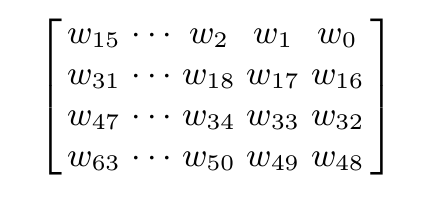
\includegraphics[width=\textwidth]{Screenshot 2024-11-30 124138.png}
        \caption*{\textbf{Cipher State}}
        \label{fig:image1}
    \end{subfigure}
    \hfill % Adds horizontal space between the images
    \begin{subfigure}[b]{0.45\textwidth} % 45% of the text width for the second image
        \centering
        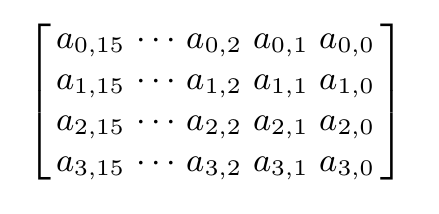
\includegraphics[width=\textwidth]{Screenshot 2024-11-30 124153.png}
        \caption*{\textbf{Subkey State}}
        \label{fig:image2}
    \end{subfigure}
    \label{fig:images}
\end{figure}
\\
\textbf{AddRoundKey(ARK)-}\\
This operation is nothing but an easy bitwise xor between
 the round subkey and the state at the intermediate of the algorithm.\\
 \begin{figure}[h!]
    \centering
    % First Image
    \begin{subfigure}[b]{1.2\textwidth}
        \centering
        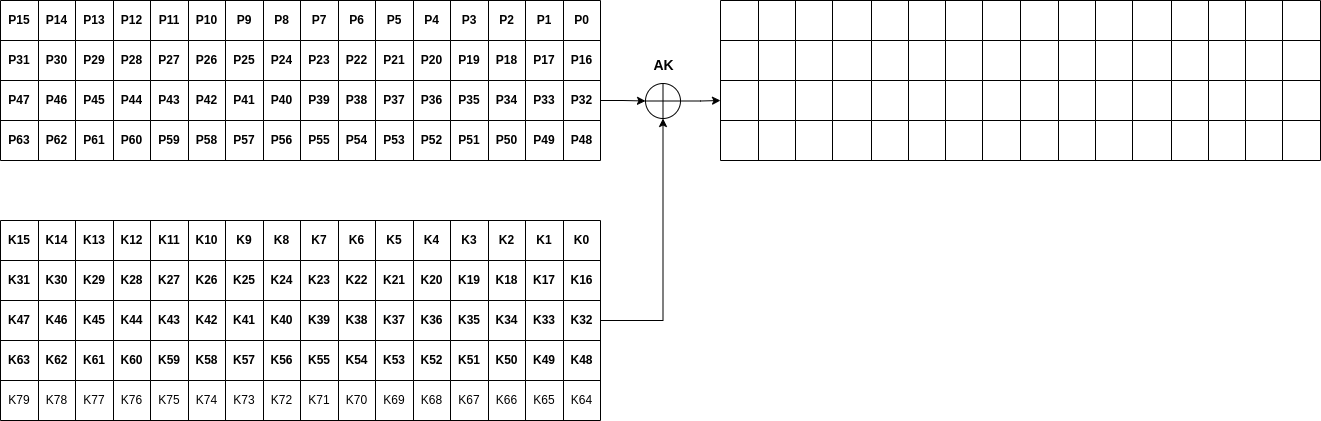
\includegraphics[width=\textwidth]{SKCrypto.drawio.png} 
        \label{fig:image1}
    \end{subfigure}
    \caption{Above diagram show add round-key operation}

\end{figure}
\\
\textbf{ SubColumn(S)-}\\
SubColumn is similar to the Subbytes operation, where the parallel application of S-boxes gets applied to the 4 bits in the same column. If the input of an S-box is Col(j) = $a_{3,j} || a_{2,j} || a_{1,j} || a_{0,j}$ for $0 \leq j \leq 15$, then the result would be S(Col(j)) = $b_{3,j} || b_{2,j} || b_{1,j} || b_{0,j}$. This operation is applied as follows-\\
\begin{figure}[H]
    \centering
    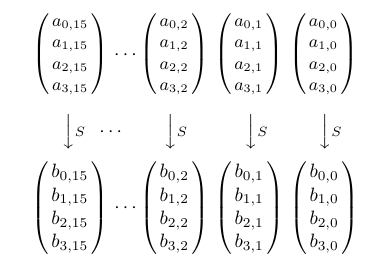
\includegraphics[width=0.4\textwidth]{Screenshot 2024-11-30 133419.png}
    \caption*{ \textbf{SubColumn Operation on the Columns of the State}}
\end{figure}

\hspace{0pt}The S-Box used in Rectangle is denoted as $F_{2}^{4} \xrightarrow{} F_{2}^{4}$  i.e. a 4-bit to 4-bit S-Box in hexadecimal which is given below in the table-
\begin{figure}[H]
    \centering
    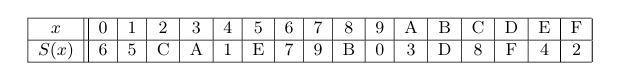
\includegraphics[width=0.8\textwidth]{Screenshot 2024-11-30 134956.png}
    \caption*{ \textbf{Rectangle Cipher S-Box}}
\end{figure}
The DDT is implemented as:
\begin{figure}[H]
    \centering
    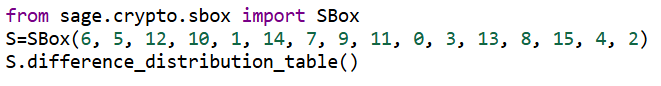
\includegraphics[width=0.7\textwidth]{Screenshot 2024-11-30 141729.png}
    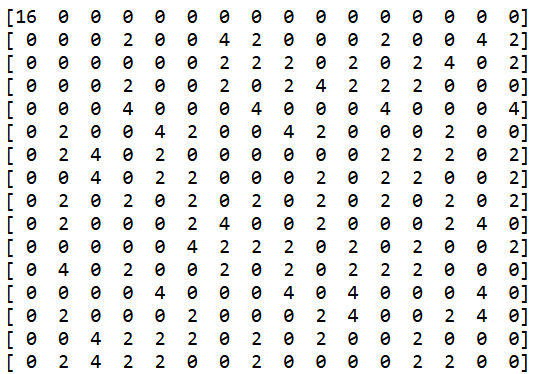
\includegraphics[width=0.7\textwidth]{Screenshot 2024-11-30 141742.png}
\end{figure}

The LAT is implemented as:
\begin{figure}[H]
    \centering
    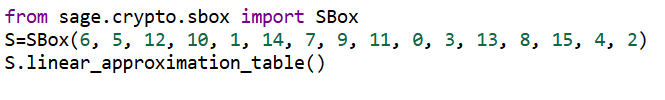
\includegraphics[width=0.7\textwidth]{Screenshot 2024-11-30 142114.png}
    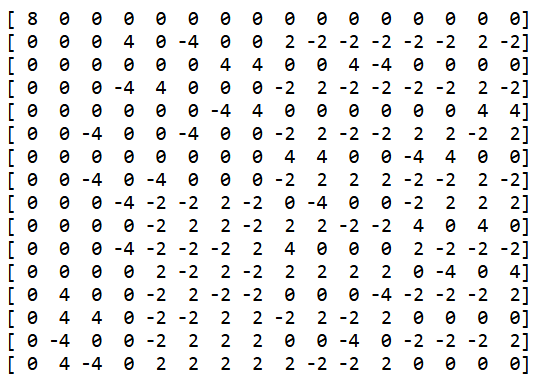
\includegraphics[width=0.7\textwidth]{Screenshot 2024-11-30 142130.png}
\end{figure}

On calculating, Differential Uniformity = 4 and Differential Branch Number = 2 for the s-box of Rectangle Cipher\\
\begin{table}[h!]
\centering
\begin{tabular}{|c|c|c|c|c|}
\hline
Group No. & Cipher Name & SBox size & Differential Uniformity & Differential Branch NUmber \\ \hline
4   & PRINCE   & 4-bit   & 4   & 2 \\ \hline
5   & KLEIN  & 4-bit   & 4   & 2  \\ \hline
6  & LED  & 4-bit  & 4  & 3  \\ \hline
8   & Midori   & 4-bit   & 4   & 2   \\ \hline
10 & GIFT  & 4-bit   & 6   & 2  \\ \hline
11  & PRINT  & 3-bit  & 2  & 2  \\ \hline
12  & Rectangle  & 4-bit  & 4  & 2  \\ \hline

\end{tabular}
\label{tab:example}
\end{table}
\\
Differential Branch Number Signifies that the greater the value , the greater the diffusion power of the permutation of SBox.\\
Our Sbox has the branch number as 2 so its not as much powerful as some of the other ciphers like LED.\\
Similarly, differential uniformity tells us the spread of the Sbox . the lower the value the more powerful the Cipher is.\\
Our uniformity value is 4 which is mostly like other
ciphers.


\textbf{ShiftRow(SR)-}\\
The ShiftRow operation involves performing left rotations on the rows of a state matrix, with varying offsets for each row. The specifics of the rotations are as follows:

Let the notation $\ll x$ represent a left rotation by $x$ bits. The transformation is illustrated below:

\[
\begin{aligned}
    &\text{Row 0:} & (a_{0,15}, \dots, a_{0,1}, a_{0,0}) & \xrightarrow{\ll 0} (a_{0,15}, \dots, a_{0,1}, a_{0,0}) \\
    &\text{Row 1:} & (a_{1,15}, \dots, a_{1,1}, a_{1,0}) & \xrightarrow{\ll 1} (a_{1,14}, \dots, a_{1,0}, a_{1,15}) \\
    &\text{Row 2:} & (a_{2,15}, \dots, a_{2,1}, a_{2,0}) & \xrightarrow{\ll 12} (a_{2,3}, \dots, a_{2,6}, a_{2,5}, a_{2,4}) \\
    &\text{Row 3:} & (a_{3,15}, \dots, a_{3,1}, a_{3,0}) & \xrightarrow{\ll 13} (a_{3,2}, \dots, a_{3,5}, a_{3,4}, a_{3,3})
\end{aligned}
\]

\begin{figure}[h!]
    \centering
    % First Image
    \begin{subfigure}[b]{1.2\textwidth}
        \centering
        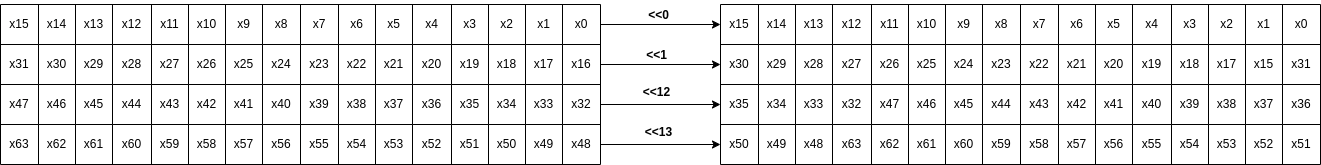
\includegraphics[width=\textwidth]{SR.drawio.png} 
        \label{fig:image1}
    \end{subfigure}
    \caption{Above diagram show shift row operation}
    \label{fig:two_images}
\end{figure}

\textbf{Key Schedule-}\\
We can have 2 types of keys with different length i.e. 80 or 128 bits\\
\textbf{Case 1: 80-bit key}\\
If the key is of 80-bit, it is represented as 5x16 rectangular array as shown in the figure below-\\

\[
\begin{bmatrix}
k_{0,15} & \cdots & k_{0,2} & k_{0,1} & k_{0,0} \\
k_{1,15} & \cdots & k_{1,2} & k_{1,1} & k_{1,0} \\
k_{2,15} & \cdots & k_{2,2} & k_{2,1} & k_{2,0} \\
k_{3,15} & \cdots & k_{3,2} & k_{3,1} & k_{3,0} \\
k_{4,15} & \cdots & k_{4,2} & k_{4,1} & k_{4,0}
\end{bmatrix}
\]


Suppose $Row_i$ = $k_{i,15}$|| ... ||$k_{i,1}$|| $k_{i,0}$ indicate the i-th key register’s row, such that 0 $\leq$ i $\leq$ 4, where $Row_i$ is considered to a sixteen bit word. At round i where i belongs to 0 to 24, the sixty-four bit round subkey $K_i$ contains the 1st 4 rows of the key register’s contents (as shown in the figure given below), i.e., $K_i = Row_3 || Row_2 || Row_1 || Row_0$.Once the key register $K_i$ found out, the key register gets updated using the following iterations-

\begin{enumerate}
\item We execute Subcolumn to the partial bits that intersect at the four uppermost rows and the four rightmost columns using the S-box S.i.e  i.e., k’3,j || k’2,j || k’1,j || k’0,j := S(k3,j || k2,j || k1,j || k0,j ), such that j belongs to (0, 1, 2, 3).\\
\item Using 1-round generalized Feistel transformation, i.e.,\\
Row'0 := (Row0 << 8) $\oplus$ Row1\\
Row'1 := Row2\\
Row'2 := Row3\\
Row'3 := (Row3 << 12) $\oplus$ Row4\\
Row'4 := Row0\\
\item  Now on the 5-bit key state (i.e. k0,4|| k0,3 || k0,2 || k0,1|| k0,0), we perform a XOR operation with RC[i] (a 5-bit round constant), i.e., k’0,4 || k’0,3 || k’0,2 || k’0,1 || k’0,0 := (k0,4|| k0,3|| k0,2|| k0,1 || k0,0) $\oplus$ RC[i]\\
Using the aforementioned iterations on the revised key state, we ultimately obtain K25. The round constants RC[i] are produced using a 5-bit LFSR for all i between 0 and 24. The five bits (rc4, rc3, rc2, rc1, rc0) are left-shifted by one bit at each round, and the new value of rc0 is then assessed as rc4 xor rc2. At the beginning, RC[0]:= 0x1 is taken. Now that we have it, we can use it to derive all the round constants (for i=0 to 24):  (0X01, 0X02, 0X04, 0X09, 0X12, 0X05,0X0B, 0X16, 0X0C, 0X19, 0X13, 0X07, 0X0F, 0X1F, 0X1E, 0X1C, 0X18, 0X11, 0X03,0X06, 0X0D, 0X1B, 0X17, 0X0E, 0X1D).
\end{enumerate}\\
\textbf{Case 2: 128-bit key}
\begin{enumerate}
    \item \textbf{Key Representation:}
    \begin{itemize}
        \item The 128-bit seed key is organized into a \(4 \times 32\) array, where each row contains 32 bits:
        \[
        \begin{bmatrix}
        \kappa_{0,31} & \cdots & \kappa_{0,1} & \kappa_{0,0} \\
        \kappa_{1,31} & \cdots & \kappa_{1,1} & \kappa_{1,0} \\
        \kappa_{2,31} & \cdots & \kappa_{2,1} & \kappa_{2,0} \\
        \kappa_{3,31} & \cdots & \kappa_{3,1} & \kappa_{3,0}
        \end{bmatrix}
        \]
        \item Each row is represented as a 32-bit word: \(\text{Row}_i = \kappa_{i,31} \| \cdots \| \kappa_{i,0}\).
    \end{itemize}
    
    \item \textbf{Subkey Extraction:}
    \begin{itemize}
        \item At each round \(i\) (\(0 \leq i \leq 24\)), the round subkey \(K_i\) is formed by extracting the 16 rightmost columns of the current key register.
    \end{itemize}
    
    \item \textbf{Key Register Update:}
    \begin{enumerate}
        \item \textbf{S-Box Transformation:}
        \[
        \kappa'_{3,j} \| \kappa'_{2,j} \| \kappa'_{1,j} \| \kappa'_{0,j} := S(\kappa_{3,j} \| \kappa_{2,j} \| \kappa_{1,j} \| \kappa_{0,j}), \quad 0 \leq j \leq 7
        \]
        
        \item \textbf{Generalized Feistel Transformation:}
        \[
        \text{Row}_0' := (\text{Row}_0 \ll 8) \oplus \text{Row}_1
        \]
        \[
        \text{Row}_1' := \text{Row}_2
        \]
        \[
        \text{Row}_2' := (\text{Row}_2 \ll 16) \oplus \text{Row}_3
        \]
        \[
        \text{Row}_3' := \text{Row}_0
        \]
        
        \item \textbf{Round Constant XOR:}
        \begin{itemize}
            \item A 5-bit round constant RC[i] is XORed with the rightmost 5 bits of Row 0:
        \[
        (\kappa_{0,4} \| \kappa_{0,3} \| \kappa_{0,2} \| \kappa_{0,1} \| \kappa_{0,0}) \oplus RC[i]
        \]

        \item The constants RC[i] (i=0,…,24) are the same as those used in the 80-bit key schedule.
        \end{itemize}
        
    \end{enumerate}
    
    \item \textbf{Final Subkey Extraction:}
    \begin{itemize}
        \item After the 24th round, the final subkey \(K_{25}\) is extracted from the updated key register.
        
    \end{itemize}
\end{enumerate}

\section{Differential Cryptanalysis}
It is the way where we observe the differences between input plaintexts and relate it to the output differences.// 
It is a kind of strong attack on the Rectangle cipher.
We know that to attack a n-bit block cipher using differential cryptanalysis there must be a difference propagation with a probablity significantly larger than $2^{1-n}$.\\
As the block size is 64 bits . so our cipher must have a difference propagation of at least $2^{-63}$ to be safe from the differential attack .\\
We know from the DDT Table that , the max differential probaility is : $2^{-6}$\\
There was a attack generated on the Rectangle cipher for upto 15 rounds . The probability of the trail of 15-rounds was found to be as : $2^{-66}$.\\
$$\begin{array}{||c|c||c|c||c|c||}
\hline \sharp R & \text { Prob. } & \sharp \mathrm{R} & \text { Prob. } & \sharp \mathrm{R} & \text { Prob. } \\
\hline 1 & 2^{-2} & 6 & 2^{-18} & 11 & 2^{-46} \\
\hline 2 & 2^{-4} & 7 & 2^{-25} & 12 & 2^{-51} \\
\hline 3 & 2^{-7} & 8 & 2^{-31} & 13 & 2^{-56} \\
\hline 4 & 2^{-10} & 9 & 2^{-36} & 14 & 2^{-61} \\
\hline 5 & 2^{-14} & 10 & 2^{-41} & 15 & 2^{-66} \\
\hline
\end{array}$$

As the ShiftRow Operation of the cipher is simple, the security of Rectangle against cryptanalysis is difficult . \\
Due to rotational symmetry every trail has upto 16 variants . For a 15 round algorithm , the differential probability lies between $2^{-66}$ to $2^{-76}$.\\

So after some experimental data, we get that it is impossible to construct an effective 15 round differential attack (distinguisher) . 4 more rounds are required to attain full dependency. Hence 25 rounds were made fixed for the RECTANGLE cipher to resist the attack . 



.
The value of differential branch number was = 2 and differntial uniformity = 4.
\section{Integral Cryptanalysis}
Integral cryptanalysis relies on analyzing how sums (or XORs) of many values propagate through the rounds of a cipher.\\\\
We design \textbf{4-round intergral distinguisher} in following way:

\begin{itemize}
    \item Choose two plaintexts $P$ and $P^*$ such that:
\[
P_{2,0} = P_{3,0} = 0 \quad \text{and} \quad P^*_{2,0} = P^*_{3,0} = 1.
\]
\begin{figure}[h!]
    \centering
    % First Image
    \begin{subfigure}[b]{0.6\textwidth}
        \centering
        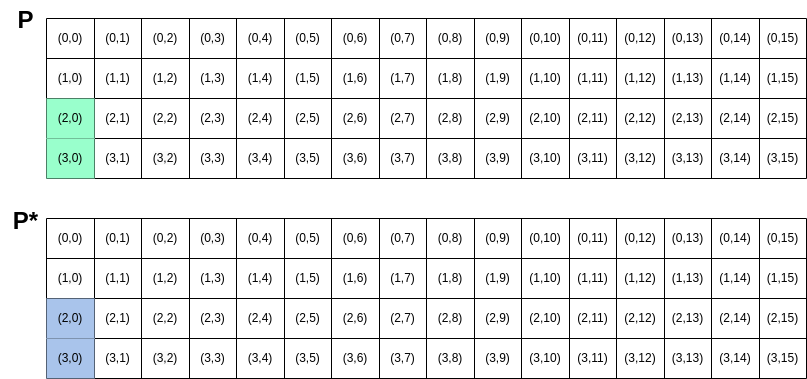
\includegraphics[width=\textwidth]{pt.drawio.png} % Replace 'image1.png' with your image filename
        \label{fig:image1}
    \end{subfigure}
\end{figure}

The other 62 bits of $P$ and $P^*$ are randomly fixed to a constant value, i.e., they follow constant property.
\begin{figure}[h!]
    \centering
    % First Image
    \begin{subfigure}[b]{0.6\textwidth}
        \centering
        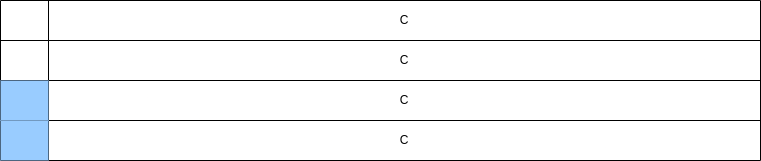
\includegraphics[width=\textwidth]{all1.drawio.png} % Replace 'image1.png' with your image filename
        \label{fig:image1}
    \end{subfigure}
\end{figure}

The difference between $P$ and $P^*$ is non-zero only in column 0:
\[
P_{\text{Col}(0)} \oplus P^*_{\text{Col}(0)} = 1100.
\]

\item Encrypt $P$ and $P^*$ through the cipher for 4 rounds:

After 4 rounds, the XOR difference of the outputs in certain positions equals 0 deterministically. These positions are:
\[
(0, 0), (1, 1), (2, 12), (3, 13)
\]
\end{itemize}


\textbf{Conclusion:}\\
At the end of 4 rounds, the XOR sum of the intermediate outputs at these bit positions is zero,i.e., they follow balanced property. This forms a 4-round integral distinguisher.\\\\
\textbf{Extending to 7 Rounds Using Decryption}
\begin{itemize}
    \item We construct a set of $2^{48}$ plaintexts where:
\begin{itemize}
    \item Certain values in columns 0, 13, 14, and 15 are fixed.
    \item The remaining 12 columns take all possible $2^{48}$ combinations,i.e., they follow All property.
\end{itemize}
\begin{figure}[h!]
    \centering
    % First Image
    \begin{subfigure}[b]{0.6\textwidth}
        \centering
        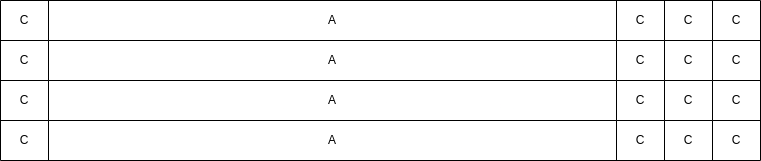
\includegraphics[width=\textwidth]{all2.drawio.png} % Replace 'image1.png' with your image filename
        \label{fig:image1}
    \end{subfigure}
\end{figure}
\item{After encrypting the $2^{48}$ plaintexts through 3 rounds, the intermediate values form $2^{47}$ subsets. Each subset contains two values that satisfy the data condition of the 4-round integral distinguisher.
\item After encrypting for 7 rounds, the XOR sum of the outputs in the same 4 bit positions remains 0:
\[
(0, 0), (1, 1), (2, 12), (3, 13)
\]
\end{itemize}
\begin{figure}[h!]
    \centering
    % First Image
    \begin{subfigure}[b]{0.6\textwidth}
        \centering
        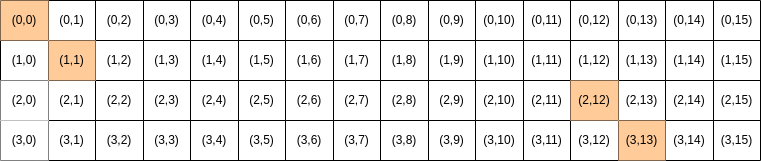
\includegraphics[width=\textwidth]{diff1.drawio.png} % Replace 'image1.png' with your image filename
        \label{fig:image1}
    \end{subfigure}
\end{figure}
\section{Software Implementation}
We have implemented Rectangle cipher on 64-bit operating system with a python interpreter.\\
\textbf{Cipher Implementation: }\\
We have designed RECTANGLE cipher for vector 4 16-bit words,and a key vector of 5 16-bit word.\\
We are taking input in hex format and printing it into binary format\\
If input have less than 64 bits then padding of 0 is added in the end.\\
Along with that a decryptor function that takes input as ciphertext and key is also made which returns us the plaintext back .

\textbf{Below are the screenshots of the terminal-}\\

\begin{figure}[htp]
    \centering
    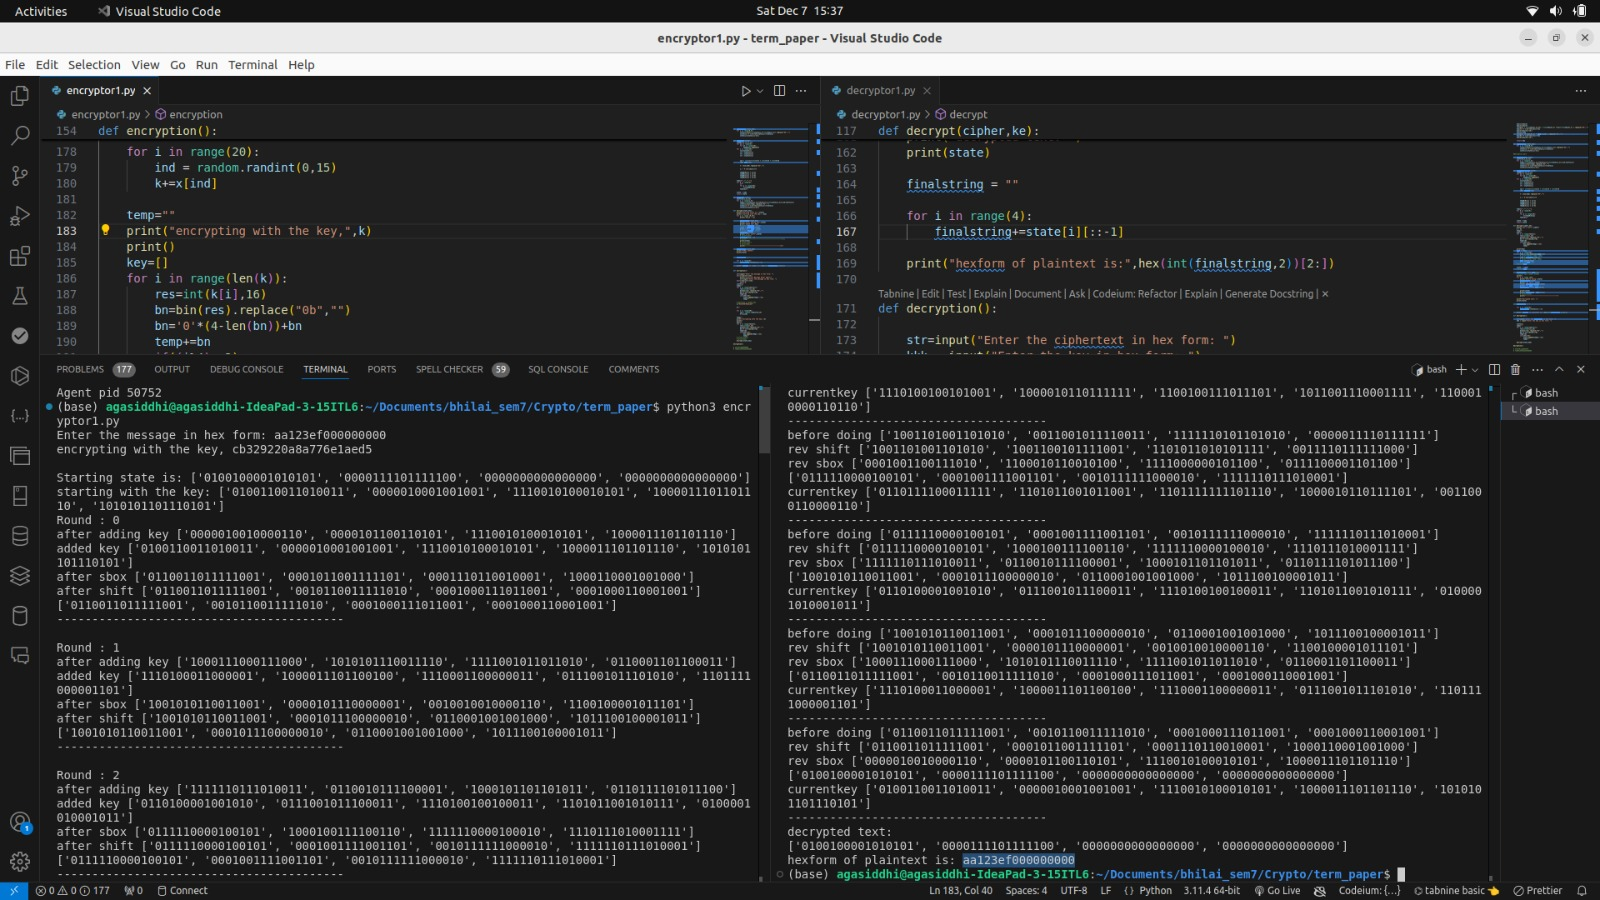
\includegraphics[height=7cm]{encryptor.jpg}
\end{figure}


\begin{figure}[htp]
    \centering
    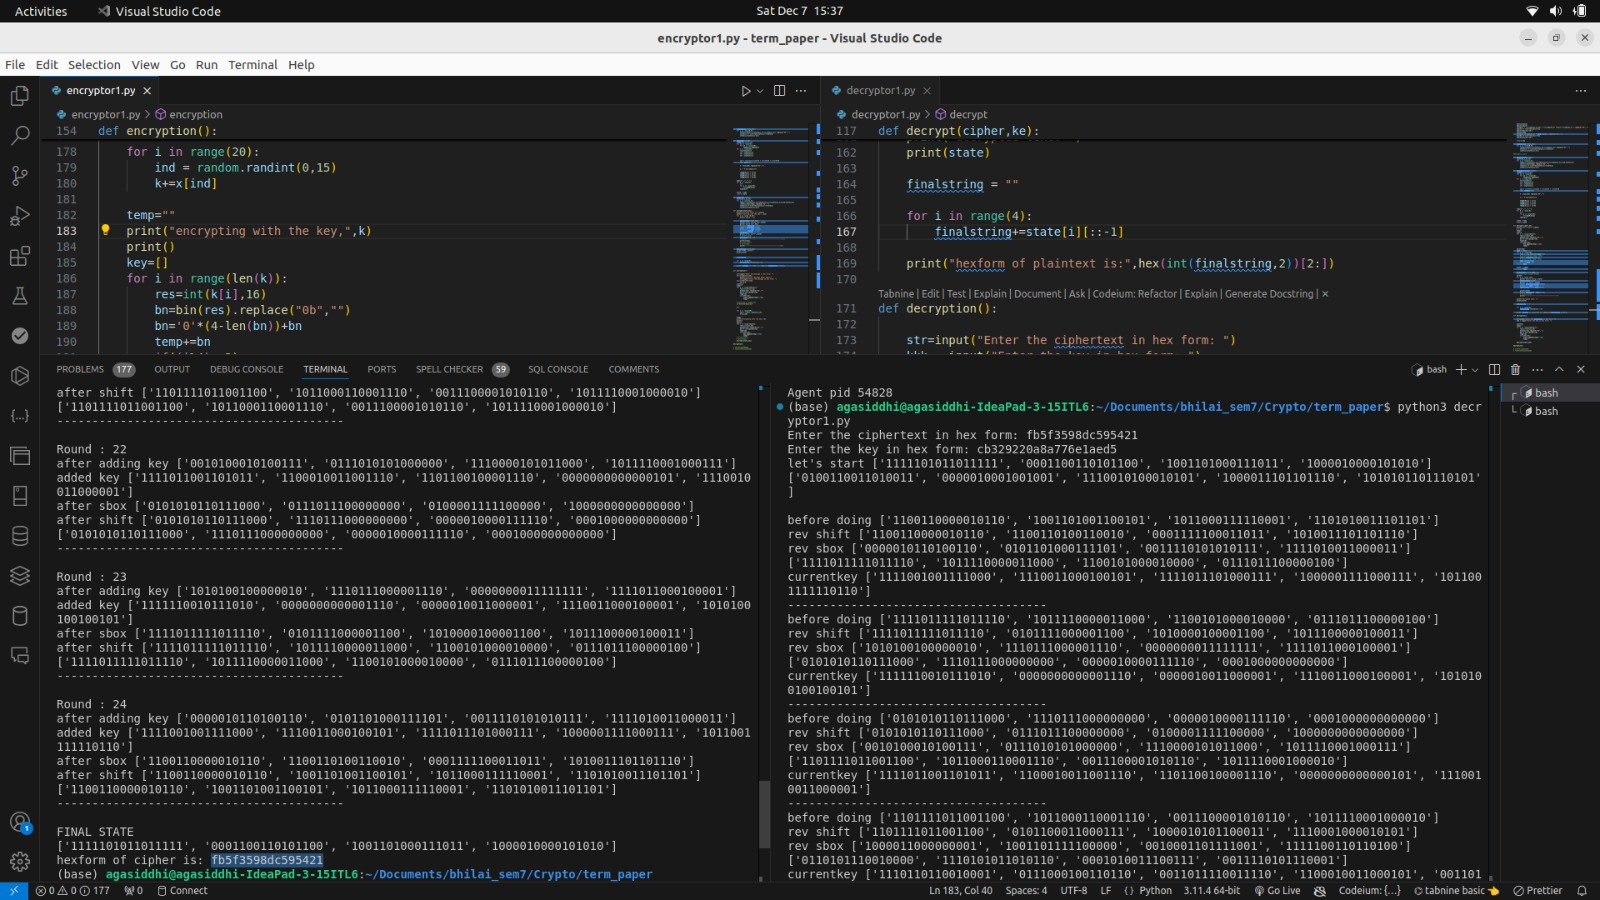
\includegraphics[width=10cm]{encryptor-2.jpg}
\end{figure}

\begin{figure}[htp]
    \centering
    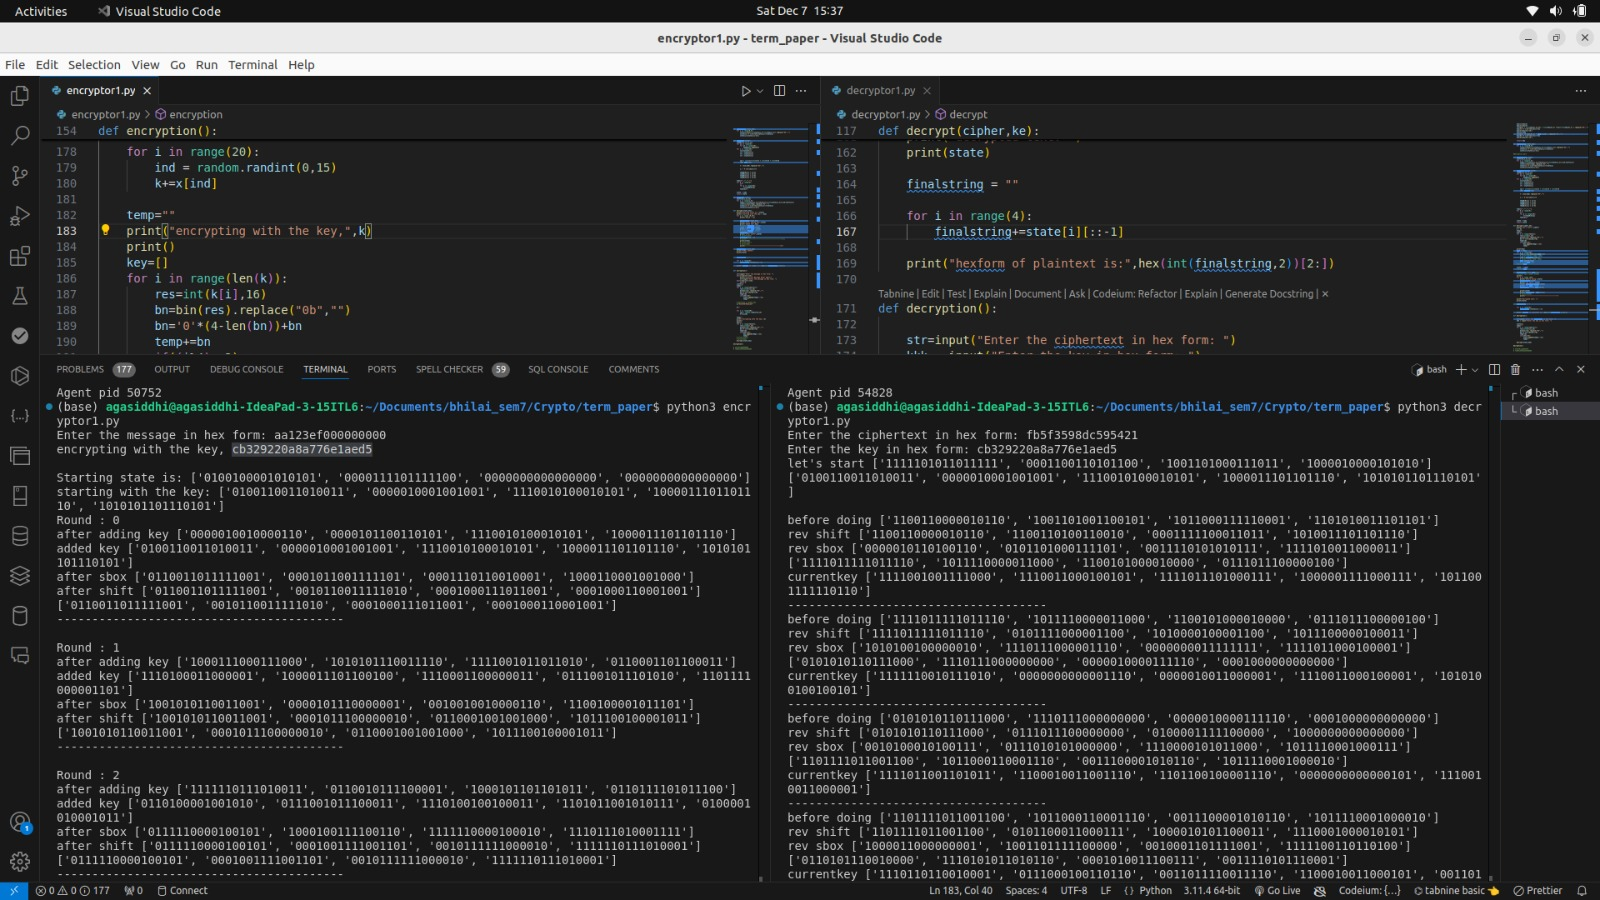
\includegraphics[width=10cm]{decryptor.jpg}
\end{figure}


\section{Application}
 Encrypt message in QR codes using RECTANGLE
    \begin{itemize}
        \item encryptor.py - contains the encryption of RECTANGLE cipher 
        \item decryptor.py - contains the decryption of RECTANGLE cipher
        \item generate\_qr.py - encrypts the message and embeds it in QR code
        \item decrypt\_qr.py - scans and retrieves the plaintext from the QR-code
    \end{itemize}
    



    \begin{figure}[h!]
    \centering
    % First Image
    \begin{subfigure}[b]{0.45\textwidth}
        \centering
        
\includegraphics[width=\textwidth]{message.png} % Replace 'image1.png' with your image filename
        \label{fig:image1}
    \end{subfigure}
    \hfill
    % Second Image
    \begin{subfigure}[b]{0.45\textwidth}
        \centering
        
\includegraphics[width=\textwidth]{birth.png} % Replace 'image2.png' with your image filename
        \label{fig:image2}
    \end{subfigure}

    \caption{Above QR Codes contain encrypted messages}
    \label{fig:two_images}
\end{figure}

\section{Conclusion}
The RECTANGLE cipher is a lightweight block cipher designed with a bit-slice technique based on an SP-network, enabling efficient and fast execution. Its design achieves exceptional performance in both software and hardware environments, making it highly adaptable for various applications. The cipher incorporates 16 parallel 4×4 S-Boxes in its substitution layer and employs three rotations in the permutation layer. This structure ensures low-cost implementation in hardware and competitive speed in software.\\
RECTANGLE's strong security performance stems from the deliberate selection of its S-Boxes and the asymmetric design of its permutation layer. Its simple yet innovative design has the potential to inspire new challenges and advancements in cryptography. Overall, the RECTANGLE cipher offers a robust combination of flexibility, efficiency, and security, making it a noteworthy contribution to the field.
\section{References}
\begin{itemize}
    \item  Research Paper source- \href{https://eprint.iacr.org/2014/084.pdf}{https://eprint.iacr.org/2014/084.pdf}
\end{itemize}

% %%%% 8. BILBIOGRAPHY %%%%
% \bibliographystyle{alpha}
% \bibliography{abbrev3,crypto,biblio}
% %%%% NOTES
% % - Download abbrev3.bib and crypto.bib from https://cryptobib.di.ens.fr/
% % - Use bilbio.bib for additional references not in the cryptobib database.
% %   If possible, take them from DBLP.

\end{document}
